\subsection{\abbr{TOF} Fiducial Cuts}\label{sec:analysis.tof_fid}

The efficiency for the \abbr{TOF} subsystem, described in Sec.~\ref{sec:clas.tof}, is different for each paddle for each section. As a result, there are regions of detection in which are inefficient. The program \abbr{GPP}, Sec.~\ref{sec:analysis.simulation}, was constructed to account for these inefficiencies in the simulation. However the \abbr{MC} indicated a greater efficiency than we measured in the data. Therefore we measured the efficiency of \abbr{CLAS} as a function of particle angle and momentum. The particles $\pi^+$, $\pi^-$ and proton momentum and angular measurements were selected from data and \abbr{MC} to analyze these functions. When an inefficiency was observed in the data, but not the \abbr{MC}, equations were derived in $\theta$ and $\phi$ to use as a cut to account for the inefficiency. Example of such an inefficiency can be seen in Fig~\ref{fig:pos:tofcut_off}, where the top panel depicts the $\pi^+$ azimuthal angle~($\phi$) vs. polar angle~($\theta$) and the bottom panel illustrates momentum~($p$) vs. polar angle~($\theta$) for sector 3.
%\begin{table}[h!]
\begin{minipage}{\textwidth}
\begin{center}
\begin{singlespacing}

\caption[Angular Range for \abbr{TOF} Plots]{\label{tab:tof.pipsec3} Angular range for \abbr{TOF} plots}
\begin{tabular}{c|c|c}
\hline												
$\phi$ Range [$\circ$]	& $\theta$ Range [$\circ$] & Plot Panel \\ \hline 	
$90 < \phi < 120$ & $10 < \theta < 45$ & Top Left \\
$90 < \phi < 120$ & $40 < \theta < 90$ & Top Right \\
$120 < \phi < 150$ & $10 < \theta < 45$ & Middle Left \\
$120 < \phi < 150$ & $40 < \theta < 90$ & Middle Right \\
\hline												
Momentum Range [GeV]	& $\theta$ Range [$\circ$] & Plot Panel \\ \hline 
$0 < \mathrm{P} < 2$ & $10 < \theta < 90$ & Bottom \\
\hline \hline%inserts single line
\end{tabular}

\end{singlespacing}
\end{center}
\end{minipage}
\end{table}
\vspace{20pt}
%At the time of writing this manuscript, there was no reliable hypothesis for dealing with the \abbr{TOF} at the \abbr{TOF} subsystem level or \abbr{TOF} paddle level.
Fig.~\ref{fig:pos:tofcut_off} shows a band of low efficiency pertaining to a inefficient \abbr{TOF} paddle between$\approx 15^\circ < \theta < 21^\circ$. Fig.~\ref{fig:pos:tofcut_off} also shows a ``rib" like structure on the bottom plot, $\theta$ vs. $p$, which is not present in the $\pi^-$ data, therefore was not further investigated as a bad paddle. The inefficient section of sector 3 was removed in data and \abbr{MC}. The effect of this cut can be seen in Fig.~\ref{fig:pos:tofcut_on}. The statistical sample used in Fig.~\ref{fig:pos:tofcut_on} was $1/5$ of the data used to derive the cut equation shown in Fig~\ref{fig:pos:tofcut_off}. There also existed an inefficiency in sector 1. The plots showing the inefficiency along with the other 5 sectors can be found in App.~\ref{sec:app.tof_plots}. The parameters for the \abbr{TOF} cuts are listed in Tab.~\ref{tab:tof.eq}. Placing the cuts described in Tab.~\ref{tab:tof.eq} is equivalent to knocking out \abbr{TOF} paddle by ID number. The variable $\phi_s$ is $\phi$ represented in the interval of $-30\le \phi \le30$ in which the term $f_{mod}$ is the $C++$ function used to perform the operation.
\begin{table}[h!]
\begin{minipage}{\textwidth}
\begin{center}
\begin{singlespacing}

\caption[\abbr{TOF} Cut Parameters]{\label{tab:tof.eq} \abbr{TOF} cut parameters.}
\begin{tabular}{c|c|c|c}
\hline												
Sector	& $\phi [^\circ]$ & $\theta$ Upper Limit ($<=$) & $\theta$ Lower Limit ($>=$)  \\ \hline 	
1 & $\phi<0$ &  $24-\phi(26-24)/30$ & $ 21.5-\phi(23.5-21.5)/30$  \\
1 & $\phi>=0$ & $ 24+\phi(26-24)/30$ & $ 21.5+\phi(23.5-21.5)/30$  \\
3 & $\phi_{s}<0$ & $ 20.5-\phi_{s}(22.-20.5)/30$ & $ 16-\phi_{s}(17.5-16)/30$  \\
3 & $\phi_{s}>=0$ & $ 20.5+\phi_{s}(22-20.5)/30$ & $ 16.+\phi_{s}(17.5-16)/30$  \\
\hline
\multicolumn{4}{c}{$\phi_{s} = fmod(fmod((\phi+390),360),60) - 30$} \\
\hline \hline%inserts single line
\end{tabular}

\end{singlespacing}
\end{center}
\end{minipage}
\end{table}
\vspace{20pt}
%Where $\phi_{s} = fmod(fmod((\phi+390),360),60) - 30$.

%1 & $\phi<0$ &  $\theta <= 24.+((26.-24.)/-30.)\phi$ & $\theta >= 21.5+((23.5-21.5)/-30.)\phi$  \\
%1 & $\phi>=0$ & $ \theta <= 24.+((26.-24.)/30.)\phi$ & $\theta >= 21.5+((23.5-21.5)/30.)\phi$  \\
%3 & $\phi_{s}<0$ & $\theta <= 20.5+((22.-20.5)/-30.)\phi_{s}$ & $\theta >= 16.+((17.5-16.)/-30.)\phi_{s}$  \\
%3 & $\phi_{s}>=0$ & $\theta <= 20.5+((22.-20.5)/30.)\phi_{s}$ & $\theta >= 16.+((17.5-16.)/30.)\phi_{s}$  \\  
%Where $\phi_{s} = fmod(fmod((\phi+390),360),60) - 30$.


\begin{figure}[h!]\begin{center}
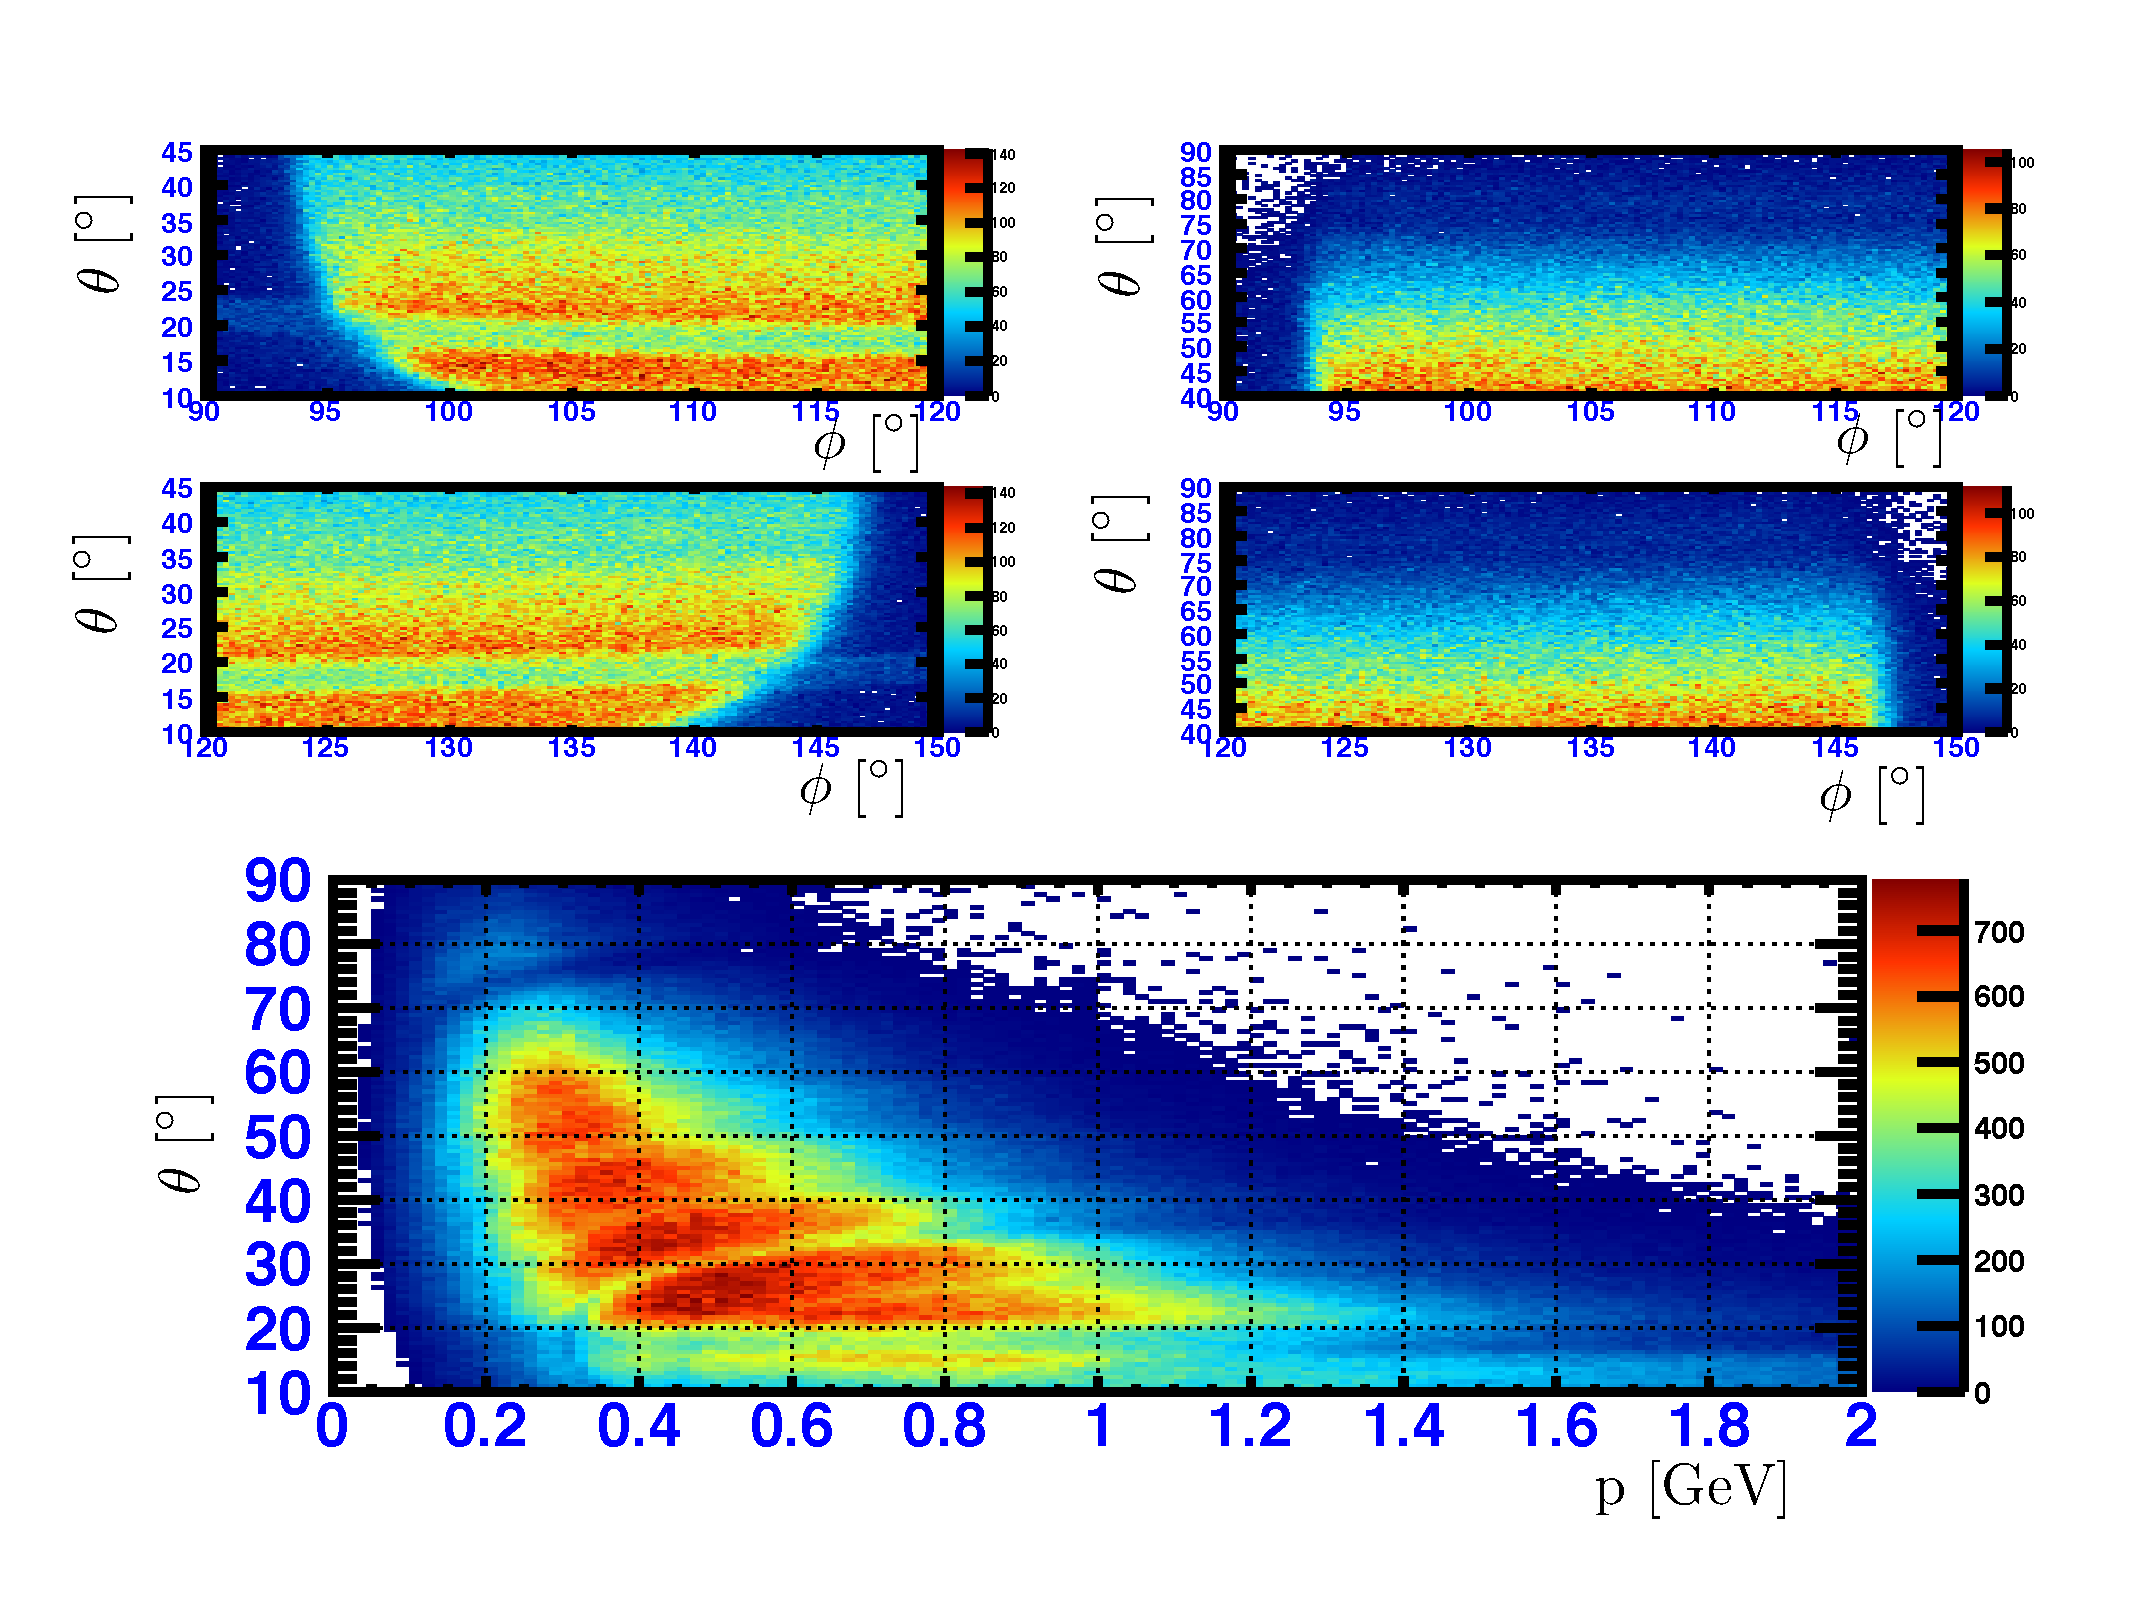
\includegraphics[width=\figwidth,height=\hfigheight]{\grpath/analysis/FIDUCIAL_CUTS/TOF/RAW/pip_sec3.pdf}
\caption[$\theta$ vs. $\phi$ of $\pi^+$ data]{\label{fig:pos:tofcut_off}(Top Left) $\theta$ vs. $\phi$ of $\pi^+$ data. Angular range $90^\circ < \phi < 120^\circ$ and $10^\circ < \theta < 45^\circ$. (Top Right) $\theta$ vs. $\phi$ of $\pi^+$ data. Angular range $90^\circ < \phi < 120^\circ$ and $40^\circ < \theta < 90^\circ$. (Middle Left) $\theta$ vs. $\phi$ of $\pi^+$ data. Angular range $120^\circ < \phi < 150^\circ$ and $10^\circ < \theta < 45^\circ$. (Middle Right) $\theta$ vs. $\phi$ of $\pi^+$ data. Angular range $120^\circ < \phi < 150^\circ$ and $40^\circ < \theta < 90^\circ$. (Bottom) $\theta$ vs. P of $\pi^+$ data. Momentum range $0 < \mathrm{P} < 2$~GeV and $\theta$ range $10^\circ < \theta < 90^\circ$. The z-axis on all plots illustrate the yield of data used in the plot.
Inefficiency seen in \abbr{CLAS} $\pi^{+} \ $data, due to an inefficient \abbr{TOF} paddle.}
\end{center}\end{figure}
%
\begin{figure}[h!]\begin{center}
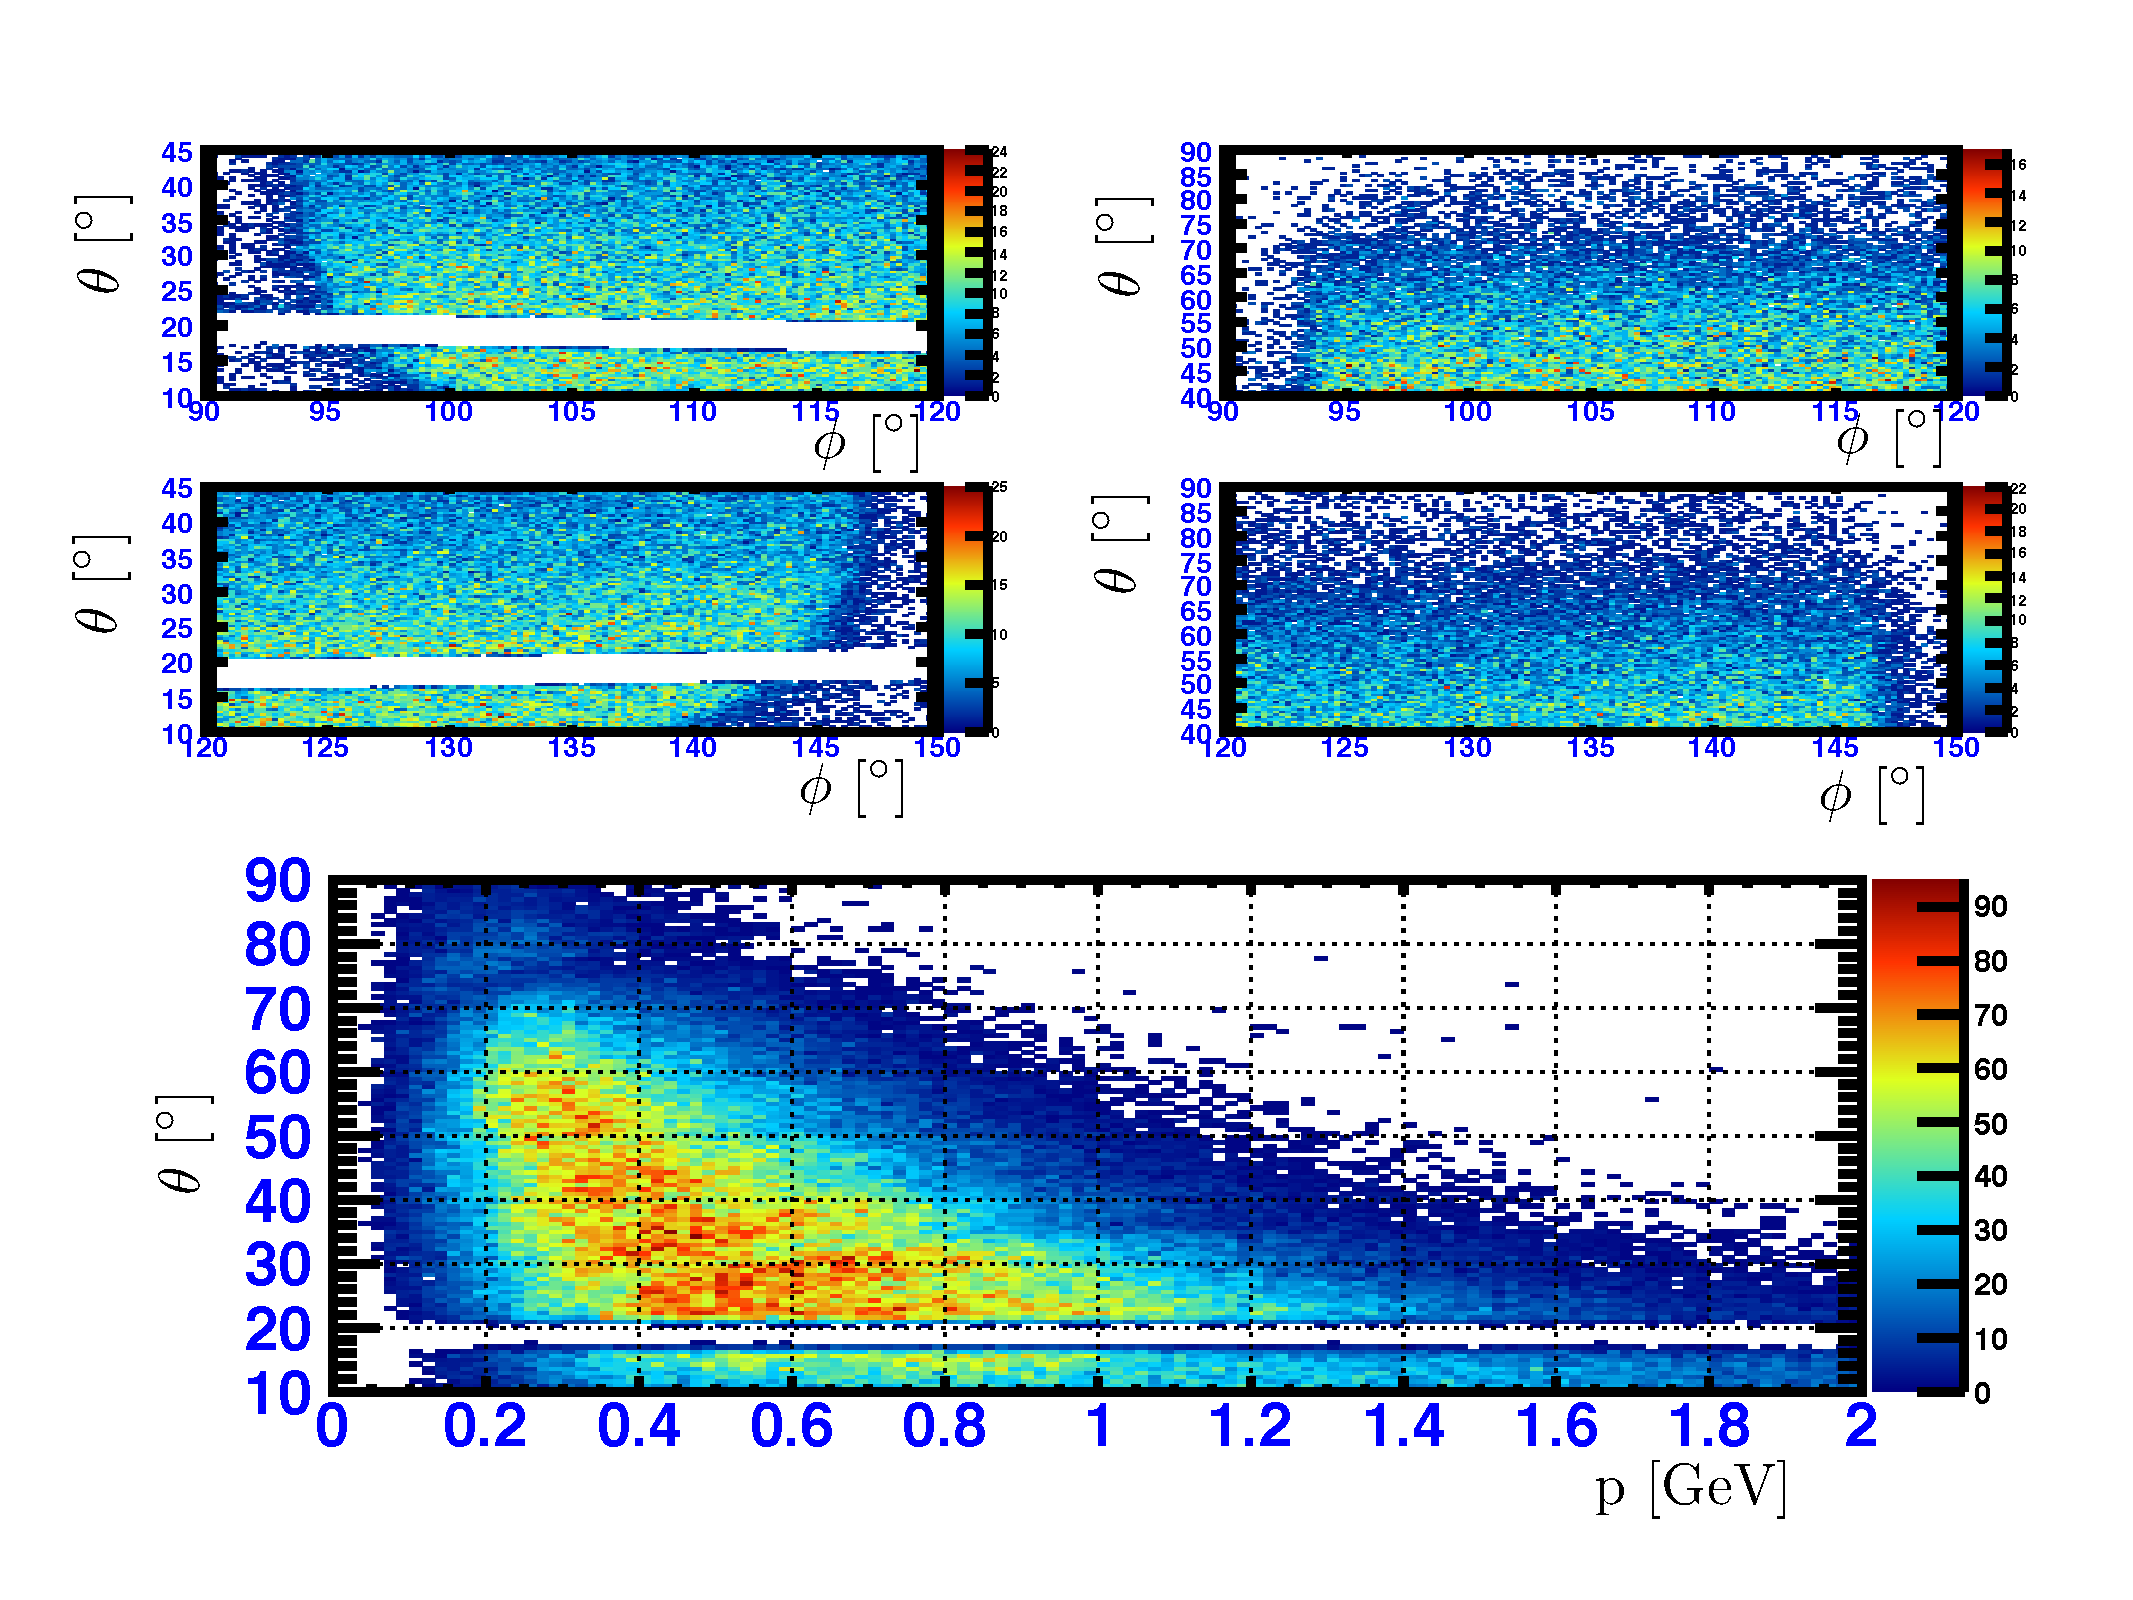
\includegraphics[width=\figwidth,height=\hfigheight]{\grpath/analysis/FIDUCIAL_CUTS/TOF/KNOCK_OUT/pip_sec3_Knockout.pdf}
\caption[Inefficiency cut for $\pi^{+} \ $ and proton data]{\label{fig:pos:tofcut_on}Inefficiency cut for $\pi^{+} \ $ and proton data. Notation same as in Fig.~\ref{fig:pos:tofcut_off}.}
\end{center}\end{figure}

\FloatBarrier